%! Tex program = xelatex
\documentclass{article}

%\usepackage[UTF8]{ctex}
\usepackage{amsmath,amssymb}
\usepackage{ntheorem}
\usepackage[letterpaper,top=2cm,bottom=2cm,left=3cm,right=3cm,marginparwidth=1.75cm]{geometry}%table package
%Table
\usepackage{multirow,booktabs}
\usepackage{makecell}
%字体颜色
\usepackage{color}
\usepackage[dvipsnames]{xcolor}  % 更全的色系
%代码
\usepackage[OT1]{fontenc}
% MATLAB 代码风格
\usepackage[framed,numbered,autolinebreaks,useliterate]{/Users/anye_zhenhaoyu/Desktop/Latex/mcode}
\usepackage{listings}
\usepackage{algorithm}
\usepackage{algorithmic}
%插图
\usepackage{graphicx}
%改变item格式
\usepackage{enumerate}
%物理
\usepackage{physics}
%extra arrows
\usepackage{extarrows}
% caption(居中指令)
%\usepackage[justification=centering]{caption}
\usepackage{caption}
% htpb
\usepackage{stfloats}
% pdf 拼接
\usepackage{pdfpages}
% 超链接url
\usepackage{url}

\def\RR{\mathbb{R}}
\def\ZZ{\mathbb{Z}}
\def\EE{\mathbb{E}}

\def\Trsp#1{#1^{\mathcal{T}}}

\def\bw{\boldsymbol{\omega}}
\def\ba{\boldsymbol{a}}
\def\bb{\boldsymbol{b}}
\def\bc{\boldsymbol{c}}
\def\bd{\boldsymbol{d}}
\def\bt{\boldsymbol{t}}
\def\bx{\boldsymbol{x}}
\def\by{\boldsymbol{y}}
\def\bz{\boldsymbol{z}}

\def\bA{\boldsymbol{A}}
\def\bB{\boldsymbol{B}}
\def\bC{\boldsymbol{C}}
\def\bE{\boldsymbol{E}}
\def\bO{\boldsymbol{O}}
\def\bX{\boldsymbol{X}}
\def\bY{\boldsymbol{Y}}

\def\Esolve{\textcolor{blue}{Solve: }}
\def\Eproof{\textcolor{blue}{Proof: }}

\def\suminf#1{\sum_{#1=-\infty}^{+\infty}}

\newtheorem{lemma}{Lemma}
\newtheorem{proof}{Proof}
\newtheorem*{theorem}{Theorem}

\graphicspath{{figures/}}


\begin{document}
\title{Homework 7}
\author{Zhen}
\maketitle

\section*{Prblem 1}
$$
\min_{x_1,x_2} f(x_1,x_2)=
e^{x_1+3x_2-0.1}+e^{x_1-3x_2-0.1}+e^{-x_1-0.1}
$$

\Esolve
\begin{enumerate}[(a)]
	\item 
		By mean value theorem:
		$$
		\begin{aligned}
			f(x_1,x_2)
			&=
			e^{-0.1}
			\qty[
				e^{x_1}\qty(e^{3x_2}+e^{-3x_2})+
				e^{-x_1}
			]
			\\&\ge
			e^{-0.1}
			\qty(2e^{x_1}+e^{-x_1})
			\\&\ge
			2\sqrt{2}e^{-0.1}
		\end{aligned}
		$$
		The equality condition is: 
		$x_2=0,x_1=-\ln\sqrt{2}$.

		Thus $\bx^*=(-\ln\sqrt{2},0)^{\mathcal{T}}$, 
		$f(\bx^*)=2\sqrt{2}e^{-0.1}$

	\item
		The output is:
		\begin{figure}[H]
			\centering
			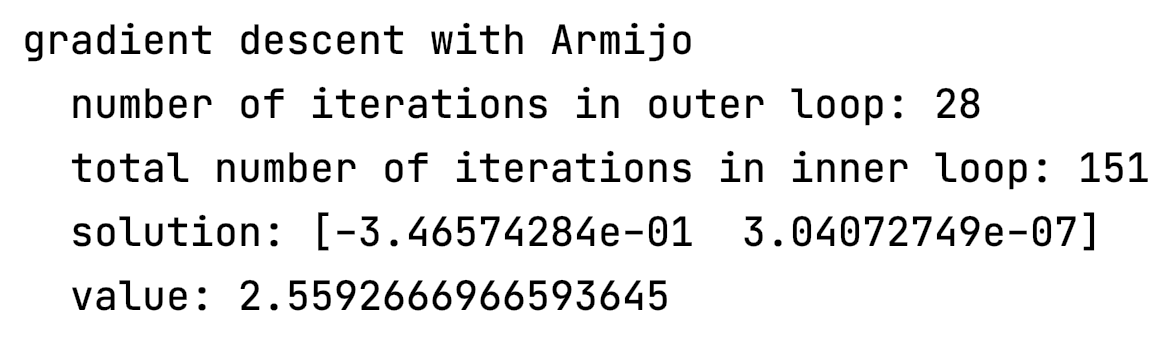
\includegraphics
			[width=0.5\linewidth]{p1bc/p1b-output.png}
		\end{figure}
		Some plots:
		\begin{figure}[h]
			\centering
			\begin{minipage}[b]{0.31\linewidth}
				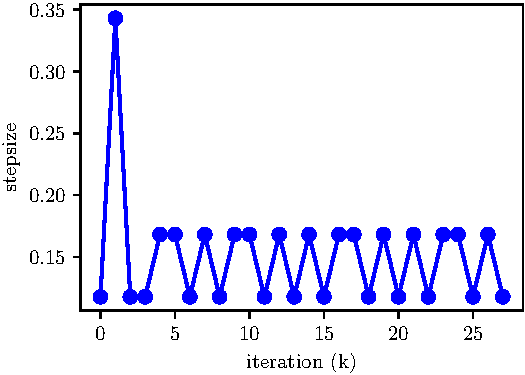
\includegraphics[width=1\linewidth]
				{p1bc/gd_armijo_ss.pdf}
				\caption*{the step sizes $t_k$}
			\end{minipage}
			\begin{minipage}[b]{0.31\linewidth}
				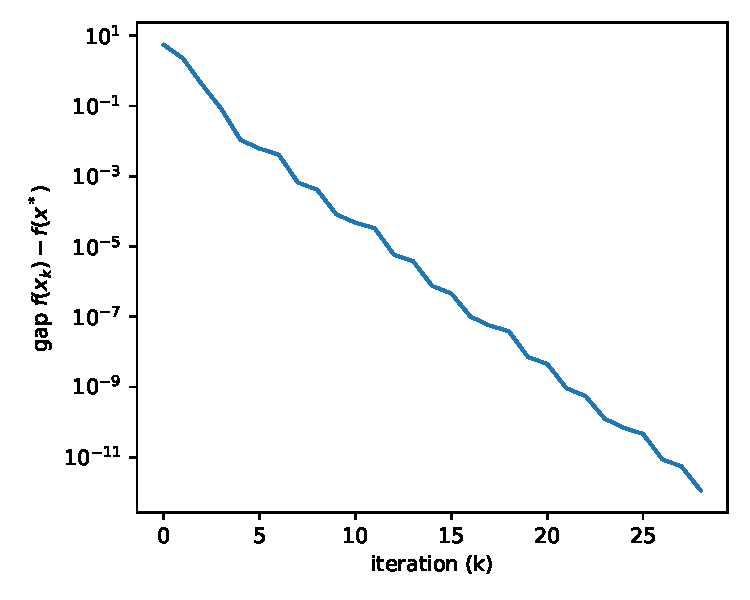
\includegraphics[width=1\linewidth]
				{p1bc/gd_error_armijo.pdf}
				\caption*{the error $f(\bx_k) - f(\bx^*)$}
			\end{minipage}
			\begin{minipage}[b]{0.31\linewidth}
			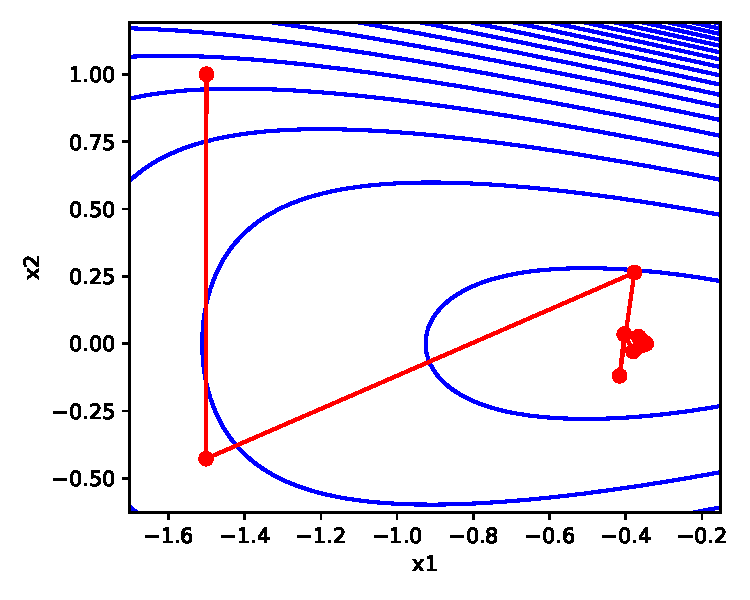
\includegraphics[width=1\linewidth]
				{p1bc/gd_traces_armijo.pdf}
				\caption*{the trajectory of $\bx_k$}
			\end{minipage}
		\end{figure}

		\newpage
	\item 
		The output is:
		\begin{figure}[H]
			\centering
			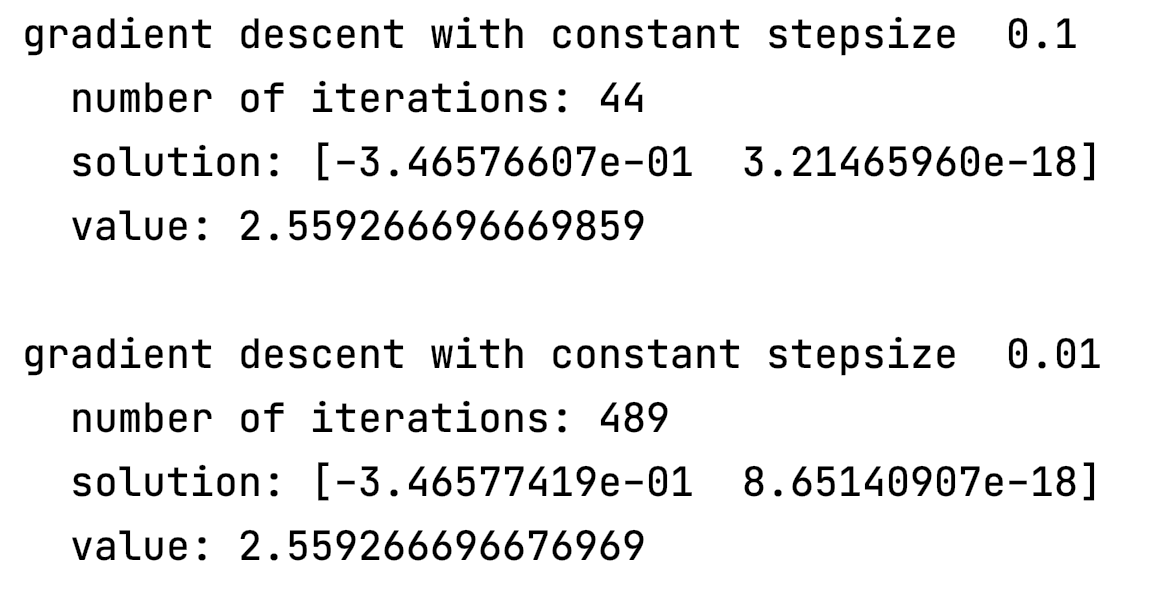
\includegraphics
			[width=0.5\linewidth]{p1bc/p1c-output.png}
		\end{figure}

		Some plots:
		\begin{figure}[h]
			\centering
			\begin{minipage}[b]{0.46\linewidth}
				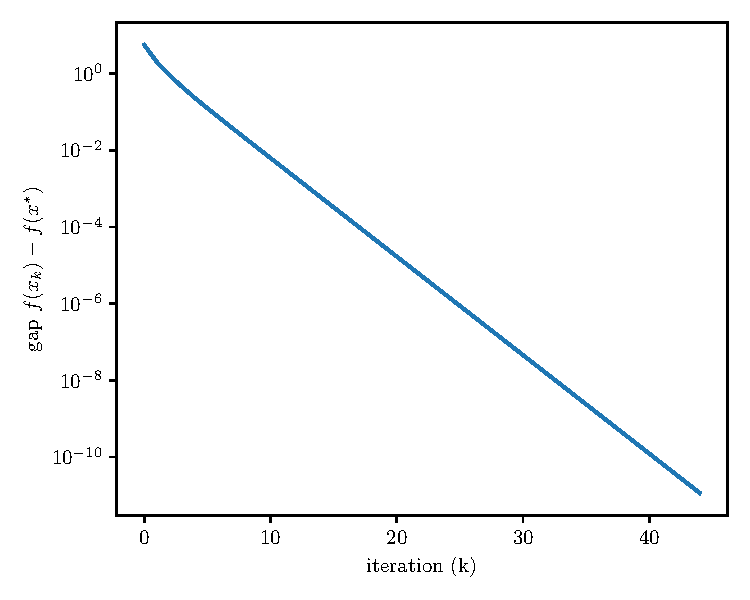
\includegraphics[width=1\linewidth]
				{p1bc/gd_error_css0.1.pdf}
				\caption*{the error $f(\bx_k) - f(\bx^*)$}
				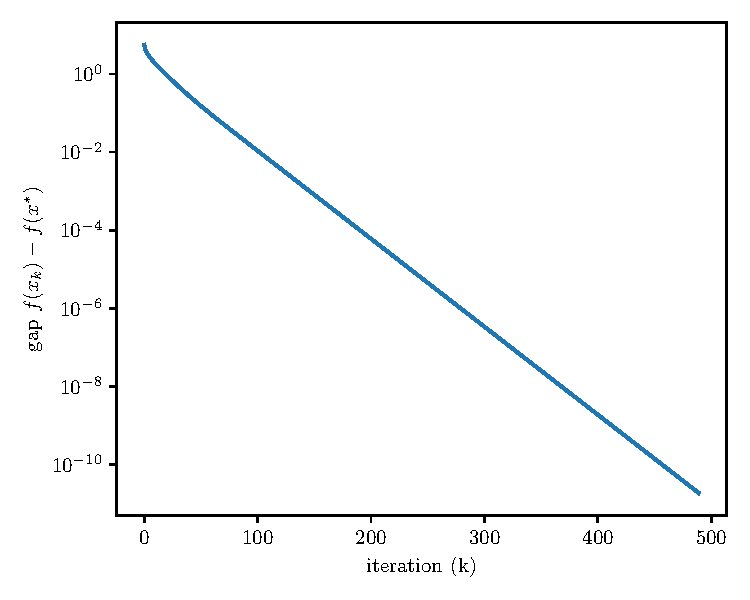
\includegraphics[width=1\linewidth]
				{p1bc/gd_error_css0.01.pdf}
				\caption*{the error $f(\bx_k) - f(\bx^*)$}
			\end{minipage}
			\begin{minipage}[b]{0.46\linewidth}
				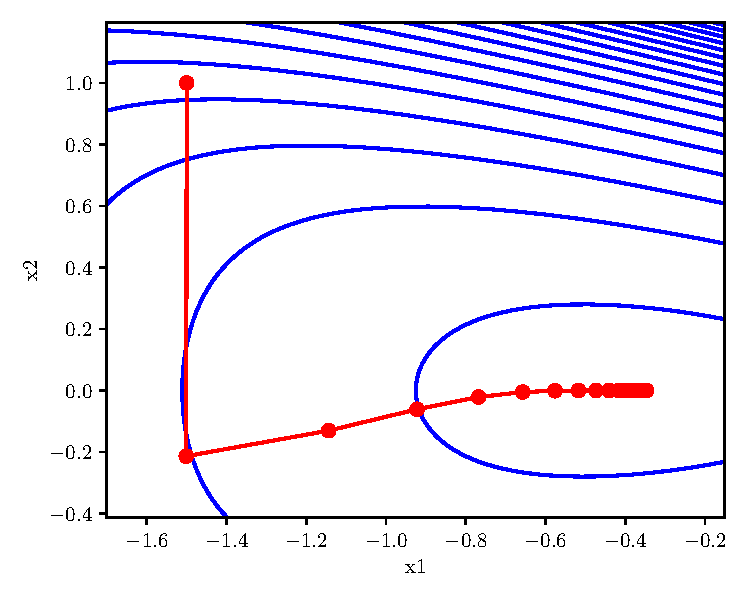
\includegraphics[width=1\linewidth]
				{p1bc/gd_traces_css0.1.pdf}
				\caption*{the trajectory of $\bx_k$}
				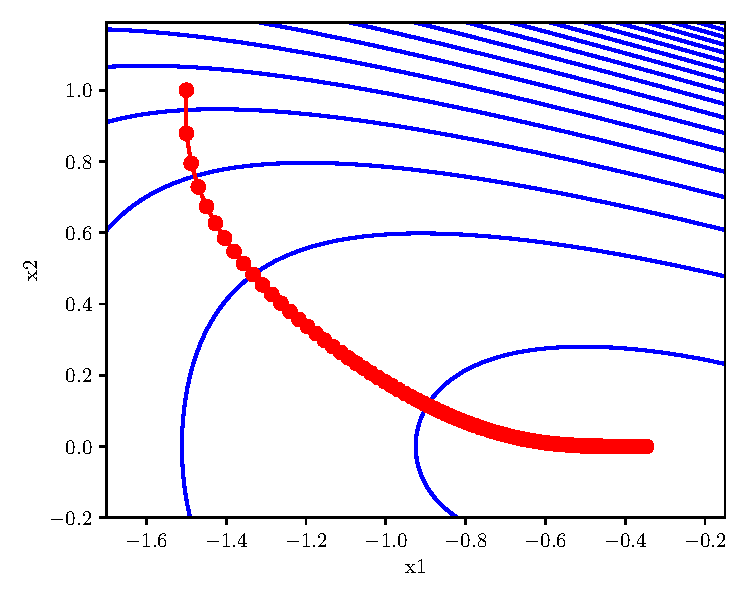
\includegraphics[width=1\linewidth]
				{p1bc/gd_traces_css0.01.pdf}
				\caption*{the trajectory of $\bx_k$}
			\end{minipage}
		\end{figure}

	\item
		The output is:
		\begin{figure}[H]
			\centering
			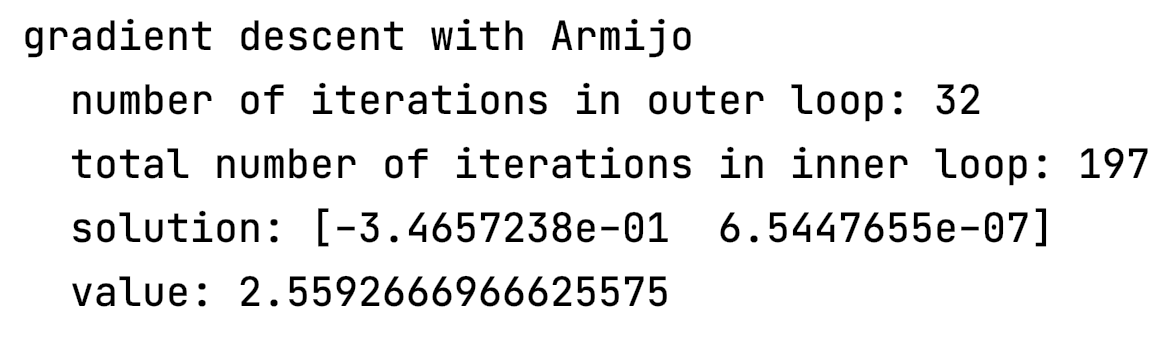
\includegraphics
			[width=0.5\linewidth]{p1de/p1d-output.png}
		\end{figure}\newpage
		Some plots:
		\begin{figure}[H]
			\centering
			\begin{minipage}[b]{0.31\linewidth}
				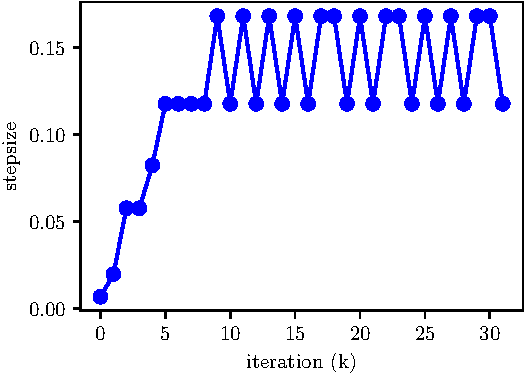
\includegraphics[width=1\linewidth]
				{p1de/gd_armijo_ss.pdf}
				\caption*{the step sizes $t_k$}
			\end{minipage}
			\begin{minipage}[b]{0.31\linewidth}
				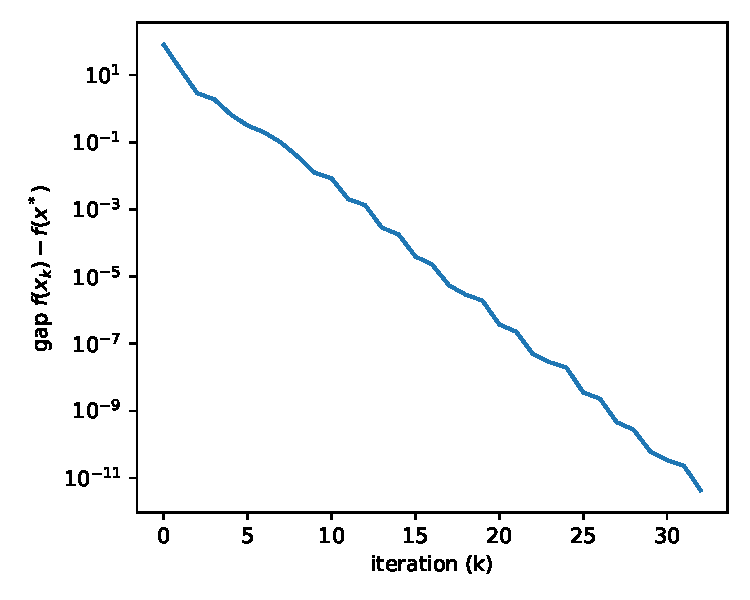
\includegraphics[width=1\linewidth]
				{p1de/gd_error_armijo.pdf}
				\caption*{the error $f(\bx_k) - f(\bx^*)$}
			\end{minipage}
			\begin{minipage}[b]{0.31\linewidth}
			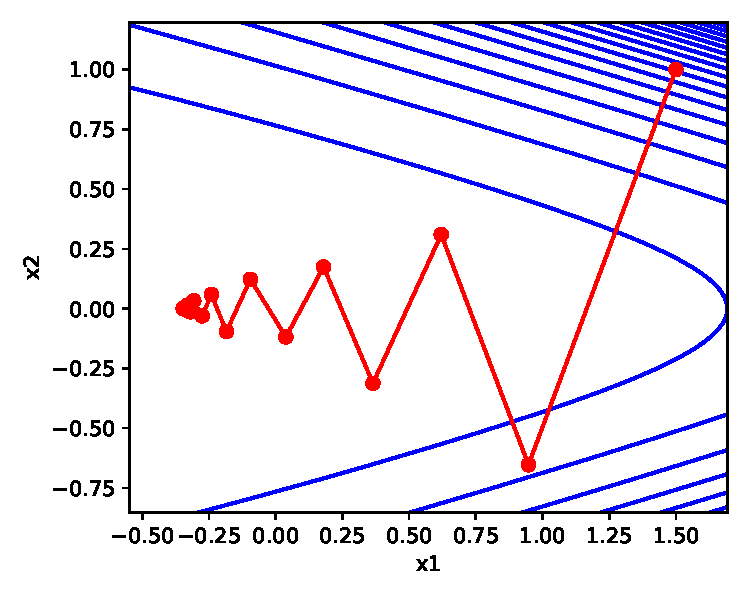
\includegraphics[width=1\linewidth]
				{p1de/gd_traces_armijo.pdf}
				\caption*{the trajectory of $\bx_k$}
			\end{minipage}
		\end{figure}
	\item
		The output is:
		\begin{figure}[H]
			\centering
			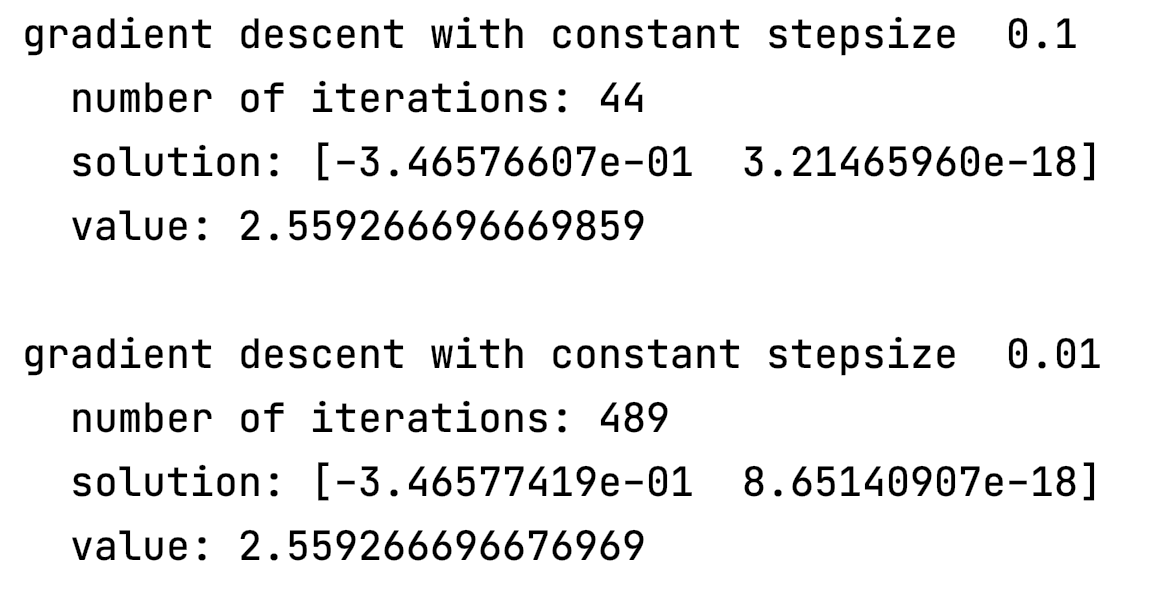
\includegraphics
			[width=0.5\linewidth]{p1bc/p1c-output.png}
		\end{figure}

		Some plots:
		\begin{figure}[H]
			\centering
			\begin{minipage}[b]{0.46\linewidth}
				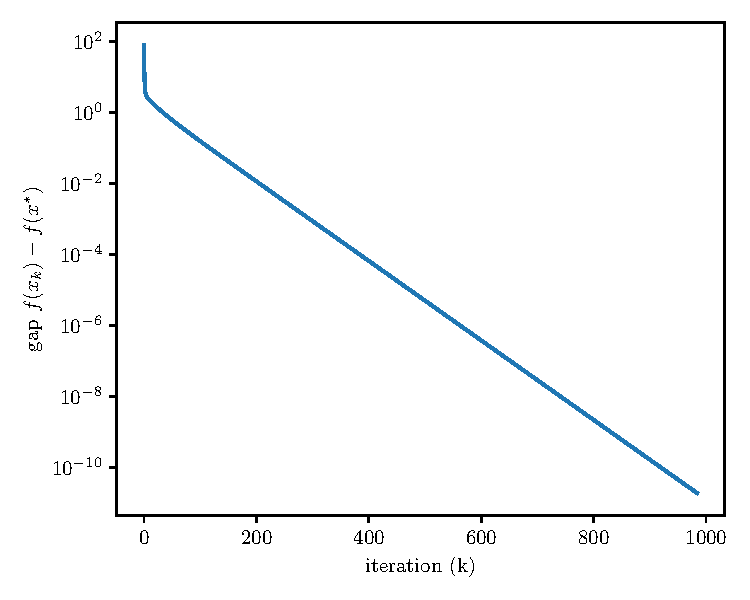
\includegraphics[width=1\linewidth]
				{p1de/gd_error_css0.005.pdf}
				\caption*{the error $f(\bx_k) - f(\bx^*)$}
			\end{minipage}
			\begin{minipage}[b]{0.46\linewidth}
				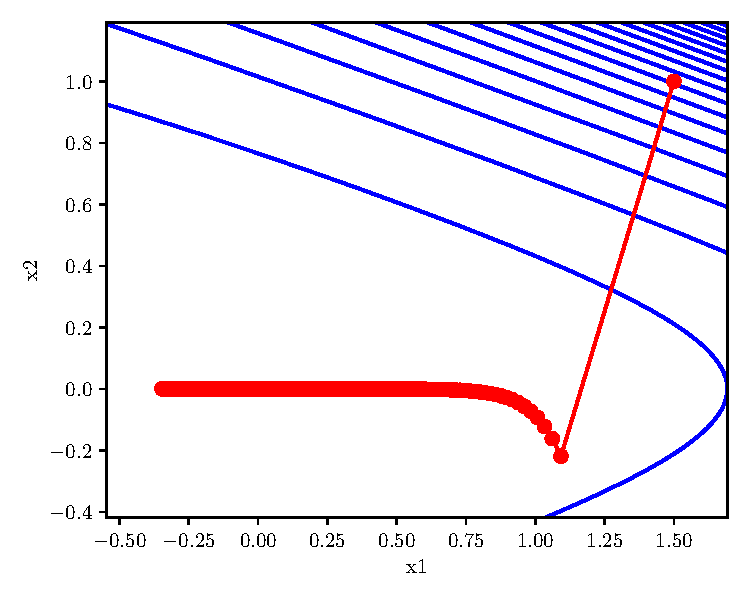
\includegraphics[width=1\linewidth]
				{p1de/gd_traces_css0.005.pdf}
				\caption*{the trajectory of $\bx_k$}
			\end{minipage}
		\end{figure}
		Using the step sizes in part (c) will generate overflow which means that the step sizes are too large and we could not get the optimal solution.
\end{enumerate}

\newpage
\section*{Prblem 2}

\textbf{Noisy gradient}: 
$$
\bx_{k+1} =
\bx_k - t(\nabla f(\bx_k) + \boldsymbol{\varepsilon}_k),
\mbox{ where }
\norm{\boldsymbol{\varepsilon}_k}\le E
$$
\Eproof
\begin{enumerate}[(a)]
	\item 
		Trivially,
		$$
		\begin{aligned}
			\norm{\bx_{k+1} - \bx^*} 
			&\le 
			\norm{\tilde{\bx}_{k+1} - \bx^*}
			+
			\norm{\bx_{k+1} - \tilde{\bx}_{k+1}}
			\\
			&=
			\norm{\tilde{\bx}_{k+1} - \bx^*}
			+
			t\norm{\boldsymbol{\varepsilon}_k}
			\\
			&\le
			\norm{\tilde{\bx}_{k+1} - \bx^*}
			+
			tE
		\end{aligned}
		$$
	
	\item
		We just need to prove: 
		$
		\norm{\tilde{\bx}_{k+1} - \bx^*}
		\le
		\sqrt{1-mt}\norm{\bx_k - \bx^*}
		$
		$$
		\begin{aligned}
			\norm{\tilde{\bx}_{k+1} - \bx^*}^2
			&=
			\norm{\bx_k - t\nabla f(\bx_k) - \bx^*}^2
			\\
			&=
			\norm{\bx_k-\bx^*}^2 + t^2\norm{\nabla f(\bx_k)}^2 
			+ 2t\nabla f(\bx_k)^{\mathcal{T}}(\bx^* - \bx_k)
			\\
			&\le
			\norm{\bx_k-\bx^*}^2 
			+ 2t\qty[f(\bx_k)-f(\bx_{k+1})]
			+ 2t\qty[f(\bx^*)-f(\bx_k)-\frac{m}{2}\norm{\bx_k-\bx^*}^2]
			\\
			&=
			(1-mt)\norm{\bx_k-\bx^*}^2+2t\qty[f(\bx^*)-f(\bx_{k+1})]
			\\
			&\le
			(1-mt)\norm{\bx_k-\bx^*}^2
		\end{aligned}
		$$
		Thus we have 
		$
		\norm{\bx_{k+1}-\bx^*}\le \sqrt{1-mt}\norm{\bx_k-\bx^*}+tE
		$.
	\item
		Apparently, 
		$\norm{\bx_0-\bx^*}\le q^0\norm{\bx_0-\bx^*}+\dfrac{1-q^0}{1-q}tE$.

		If 
		$\norm{\bx_k-\bx^*}\le q^k\norm{\bx_0-\bx^*}+\dfrac{1-q^k}{1-q}tE$, then:
		$$
		\begin{aligned}
			\norm{\bx_k-\bx^*}
			&\le
			q\norm{\bx_k-\bx^*}+tE
			\\
			&\le
			q\times
			\qty(q^k\norm{\bx_0-\bx^*}+\dfrac{1-q^k}{1-q}tE)
			+tE
			\\
			&=
			q^{k+1}\norm{\bx_0-\bx^*}+\dfrac{1-q^{k+1}}{1-q}t
		\end{aligned}
		$$
		By induction, the inequality ``$\norm{\bx_k-\bx^*}\le q^k\norm{\bx_0-\bx^*}+\dfrac{1-q^k}{1-q}tE$'' holds.

	\item
		$$
		\begin{aligned}
			\mathop{\lim\sup}_{k\to\infty}\norm{\bx_k-\bx^*}
			&\le
			\mathop{\lim\sup}_{k\to\infty}
			\qty(q^k\norm{\bx_0-\bx^*}+\dfrac{1-q^k}{1-q}tE])
			\\
			&=\frac{tE}{1-q}
			\\
			&=
			\frac{tE}{1-\sqrt{1-mt}}
			\\&\le
			\frac{tE}{1-\qty(1-mt/2)}
			\\
			&=
			\frac{2E}{m}
		\end{aligned}
		$$
\end{enumerate}

\end{document}

